%!TEX program = xelatex
% Note: this template must be compiled with XeLaTeX rather than PDFLaTeX
% due to the custom fonts used. The line above should ensure this happens
% automatically, but if it doesn't, your LaTeX editor should have a simple toggle
% to switch to using XeLaTeX.

\documentclass[
	aspectratio=169, % Uncomment to use an aspect ratio of 16:9 (160 mm by 90 mm)
	%aspectratio=43, % Uncomment to use an aspect ratio of 4:3 (128mm by 96mm)
	t, % Top align all slide content by default
	onlytextwidth, % Typeset content in columns at text width
	10pt, % Default font size, use 10pt for the 16:9 aspect ratio and 8pt for the 4:3 aspect ratio
]{beamer}

\usepackage{../ImperialTheme/beamerthemeImperial} % Use the Imperial theme

\def\imagefolder{../ImperialTheme/Images/}

\title{Domain sensitivity analysis} % Presentation title to appear on the title slide and left footers

\subtitle{} % Presentation subtitle to appear on the title slide

\author{Víctor Ballester} % Author name(s) to appear on the title slide

\date{\today} % Presentation date to appear on the title slide and right footers

\begin{document}

\begingroup
\setbeamercolor{background canvas}{bg=ICLBlue} % Slide background color
\setbeamercolor{title page title}{fg=white} % Title text color
\setbeamercolor{title page subtitle}{fg=white} % Subtitle text color
\setbeamercolor{author}{fg=white} % Author(s) text color
\setbeamercolor{date}{fg=white} % Date text color
\setbeamertemplate{title page}[logo]{\imagefolder/ICL_Logo_White.pdf} % Imperial logo color, use 'ICL_Logo_White.pdf' for white and 'ICL_Logo_Blue.pdf' for blue
\frame[plain, s]{\titlepage} % Output the title page with no footer ('plain') and vertically distributed text ('s')
\endgroup

\begin{frame}
	\frametitle{Summary}
	Our goal here is to determine the appropriate domain for which there is no dependence on the final solution in the length scales of the domain, say the $x$ distance before and after the gap and the height of the domain.

	\begin{columns}[T] % [T] ensures correct vertical alignment
		\begin{column}{0.48\linewidth} % Left column
			\textbf{Data}
			\begin{itemize}
				\item $Re_{\delta^*} = 1000$
				\item $D/\delta^* = 4$
				\item $W/\delta^* = 15$
			\end{itemize}
		\end{column}
	\end{columns}

	(for not forgetting it in the future) for Blasius profile $\delta = 2.85 \delta^*$ (if the other text books say slightly different values, it is because they are using approximations. I computed the \textbf{exact} value.)
\end{frame}
\begin{frame}
	\frametitle{Domains considered}
	Coding system: $ioh$, where $i, o, h\in \{1, 2, 3\}$ and $i$ is the inflow, $o$ is the outflow and $h$ is the height of the domain, and the numbers mean from small size (1) to large size (3).

	\small % Reduce font size in this slide
	\begin{columns}[T] % [T] ensures correct vertical alignment
		\begin{column}{0.3\linewidth} % Left column
			
\includegraphics[width=\linewidth]{Images/133.png}
			{\tiny\textcolor{ICLBlue}{133 (small inflow)}}\\[2pt]
			
\includegraphics[width=\linewidth]{Images/233.png}
			{\tiny\textcolor{ICLBlue}{233 (medium inflow)}}\\[2pt]
		\end{column}
		\begin{column}{0.3\linewidth} % Center column
			
\includegraphics[width=\linewidth]{Images/313.png}
			{\tiny\textcolor{ICLBlue}{313 (small outflow)}}\\[2pt]
			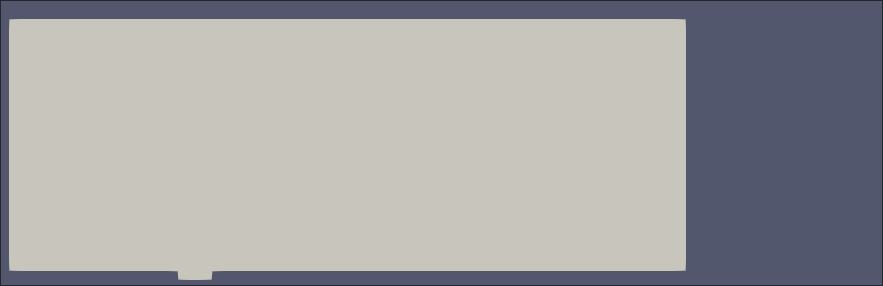
\includegraphics[width=\linewidth]{Images/323.png}
			{\tiny\textcolor{ICLBlue}{323 (medium outflow)}}\\[2pt]
			
\includegraphics[width=\linewidth]{Images/333.png}
			{\tiny\textcolor{ICLBlue}{333 (large everything)}}\\[2pt]
		\end{column}
		\begin{column}{0.3\linewidth} % Right column
			
\includegraphics[width=\linewidth]{Images/331.png}
			{\tiny\textcolor{ICLBlue}{331 (small height)}}\\[2pt]
			
\includegraphics[width=\linewidth]{Images/332.png}
			{\tiny\textcolor{ICLBlue}{332 (medium height)}}\\[2pt]
			
\includegraphics[width=\linewidth]{Images/original.png}
			{\tiny\textcolor{ICLBlue}{original domain}}\\[2pt]
		\end{column}
	\end{columns}
\end{frame}
\begin{frame}
	\frametitle{Points of interest}

	We fix some points in the domain to study their time evolution:

	\centering
	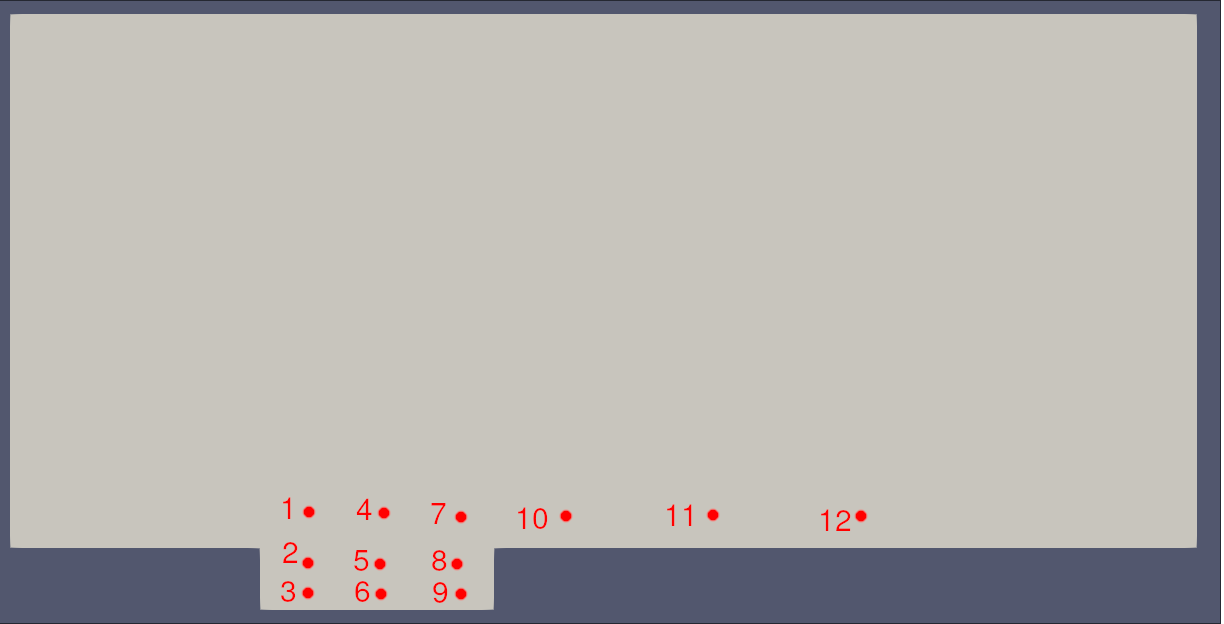
\includegraphics[width=0.8\linewidth]{Images/points.png}

\end{frame}
\begin{frame}
	\frametitle{Results}
	Point 1:

	\centering
	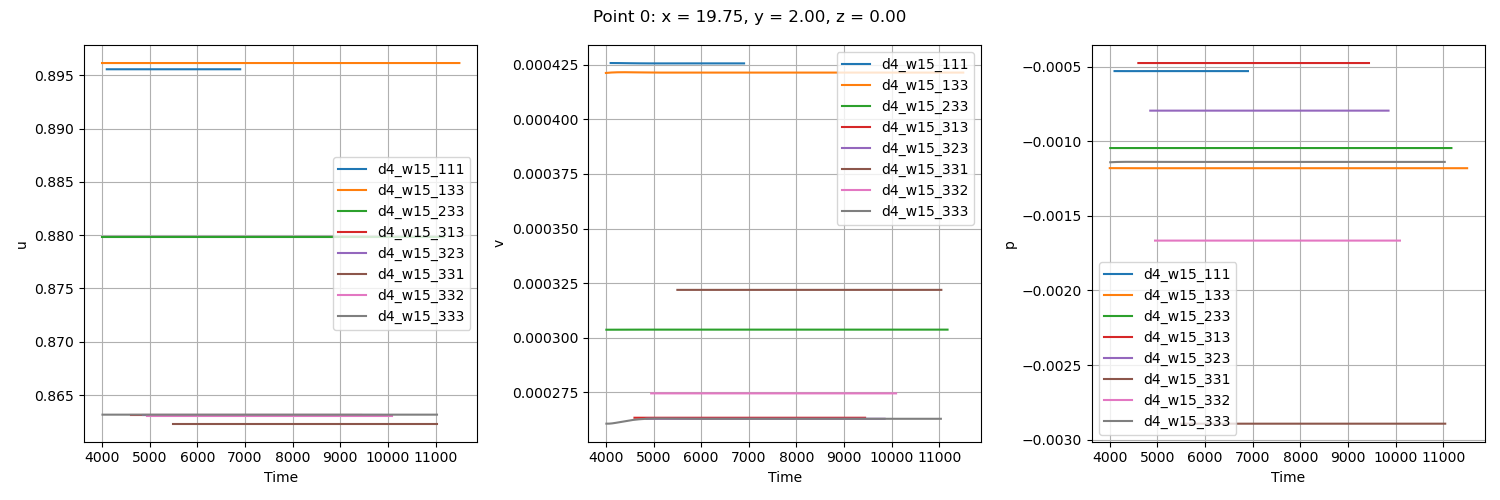
\includegraphics[width=\linewidth]{Images/point1.png}
\end{frame}
\begin{frame}
	\frametitle{Results}
	Point 2:

	\centering
	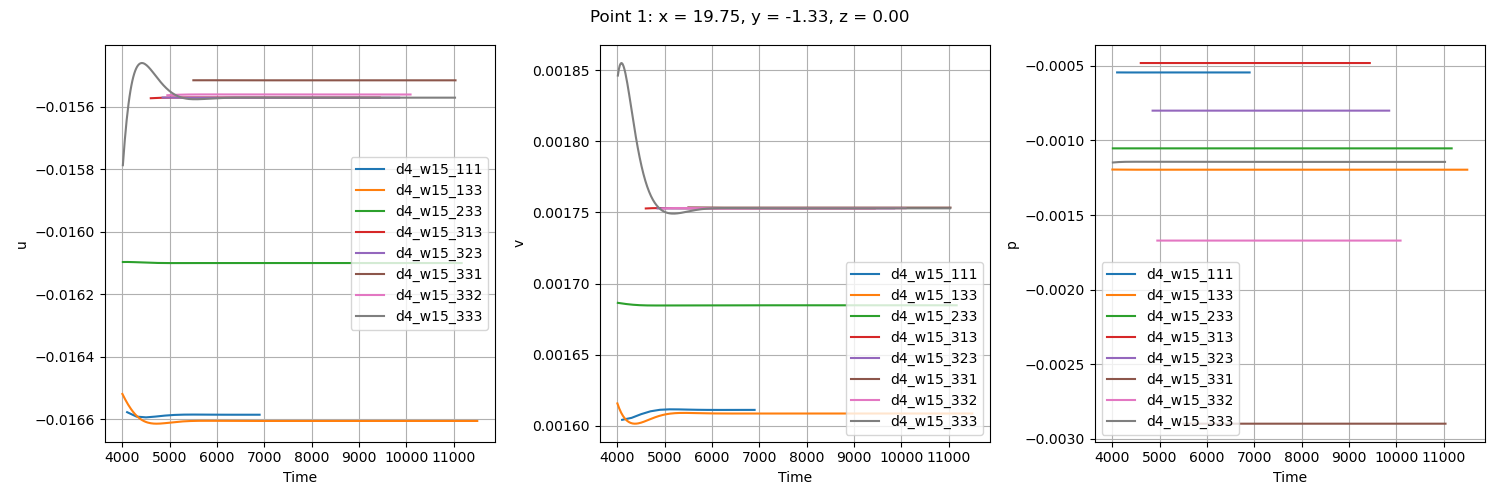
\includegraphics[width=\linewidth]{Images/point2.png}
\end{frame}
\begin{frame}
	\frametitle{Results}
	Point 3:

	\centering
	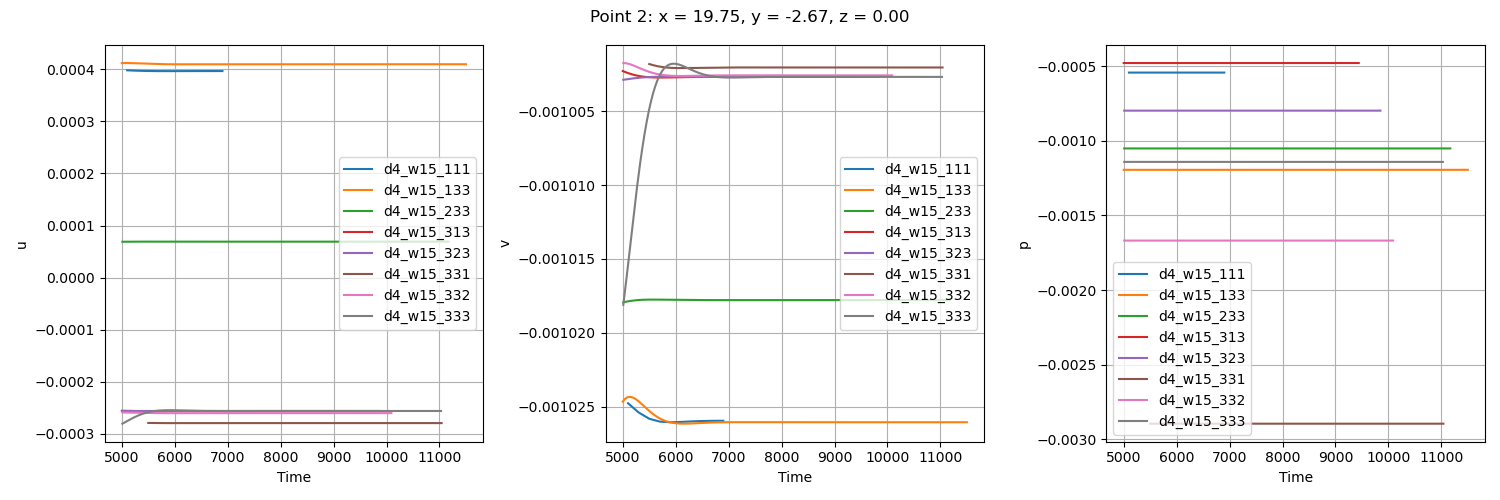
\includegraphics[width=\linewidth]{Images/point3.png}
\end{frame}
\begin{frame}
	\frametitle{Results}
	Point 4:

	\centering
	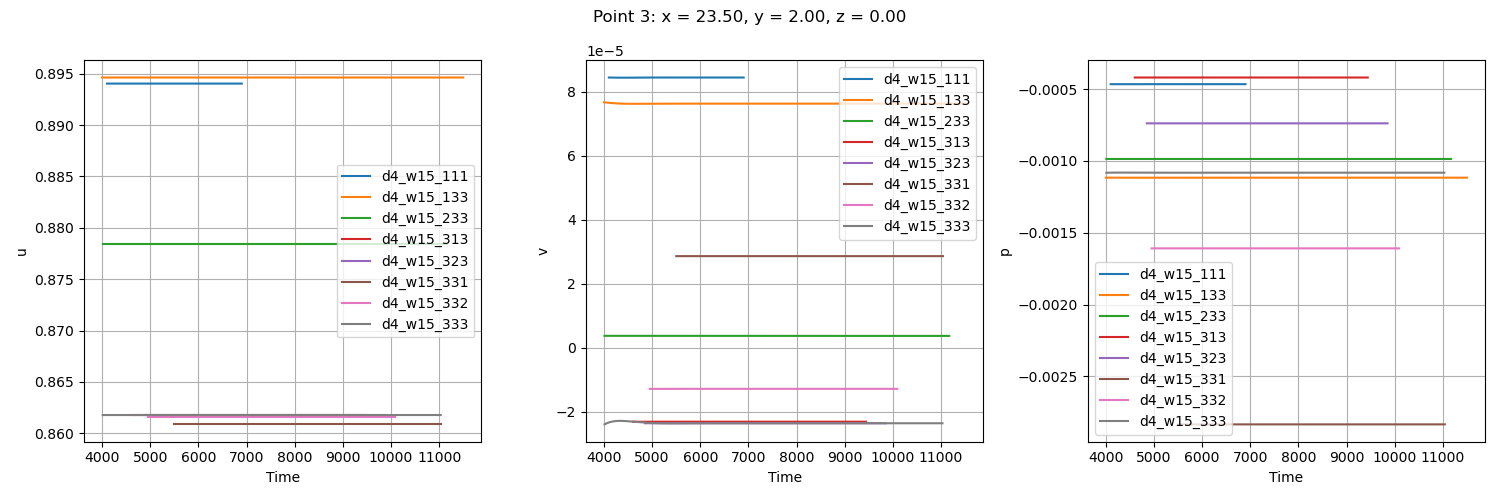
\includegraphics[width=\linewidth]{Images/point4.png}
\end{frame}
\begin{frame}
	\frametitle{Results}
	Point 5:

	\centering
	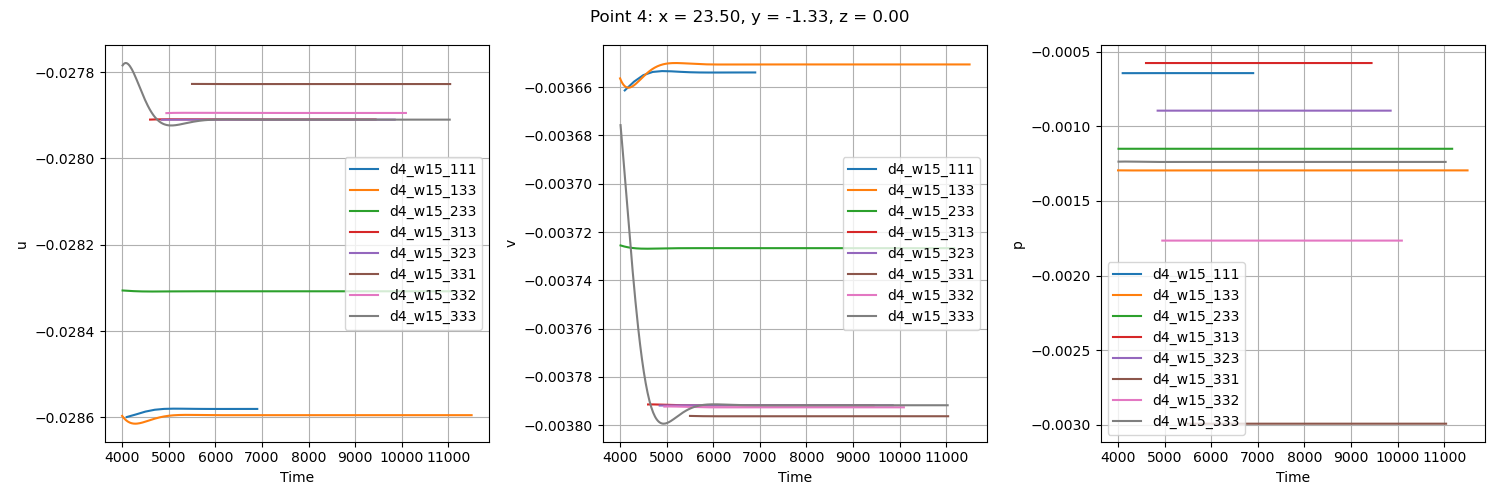
\includegraphics[width=\linewidth]{Images/point5.png}
\end{frame}
\begin{frame}
	\frametitle{Results}
	Point 6:

	\centering
	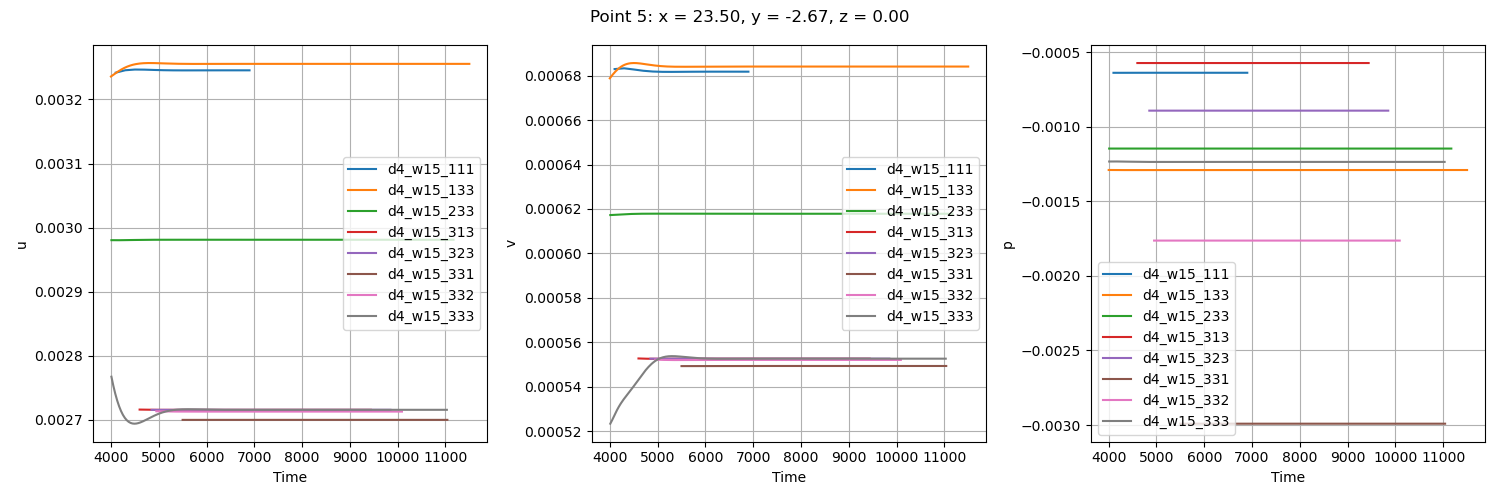
\includegraphics[width=\linewidth]{Images/point6.png}
\end{frame}
\begin{frame}
	\frametitle{Results}
	Point 7:

	\centering
	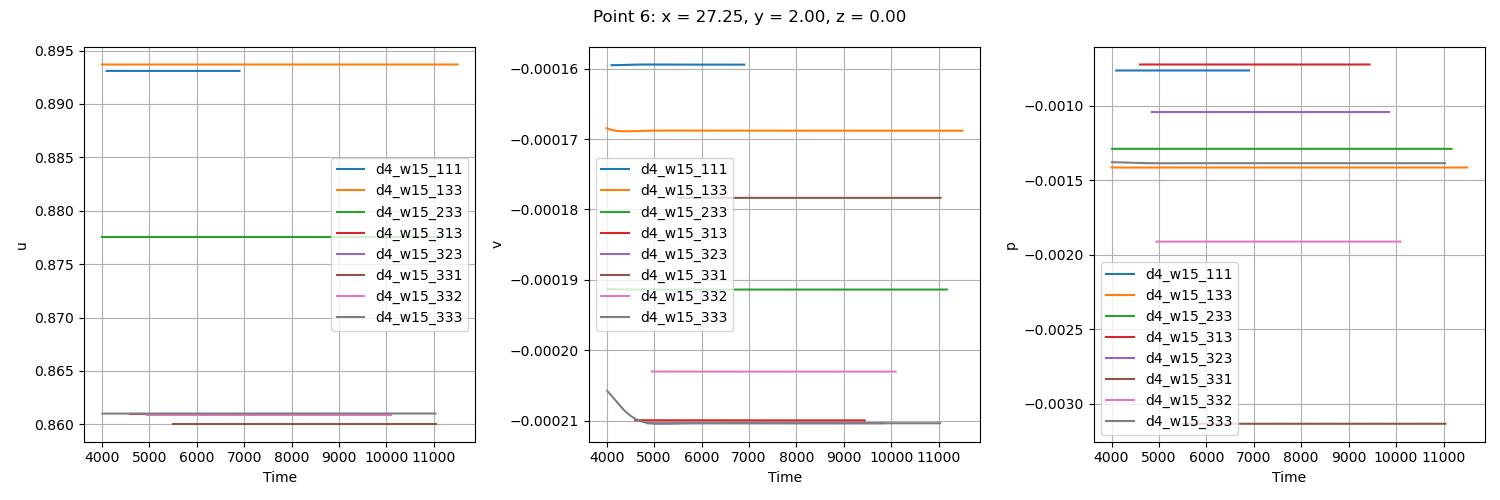
\includegraphics[width=\linewidth]{Images/point7.png}
\end{frame}
\begin{frame}
	\frametitle{Results}
	Point 8:

	\centering
	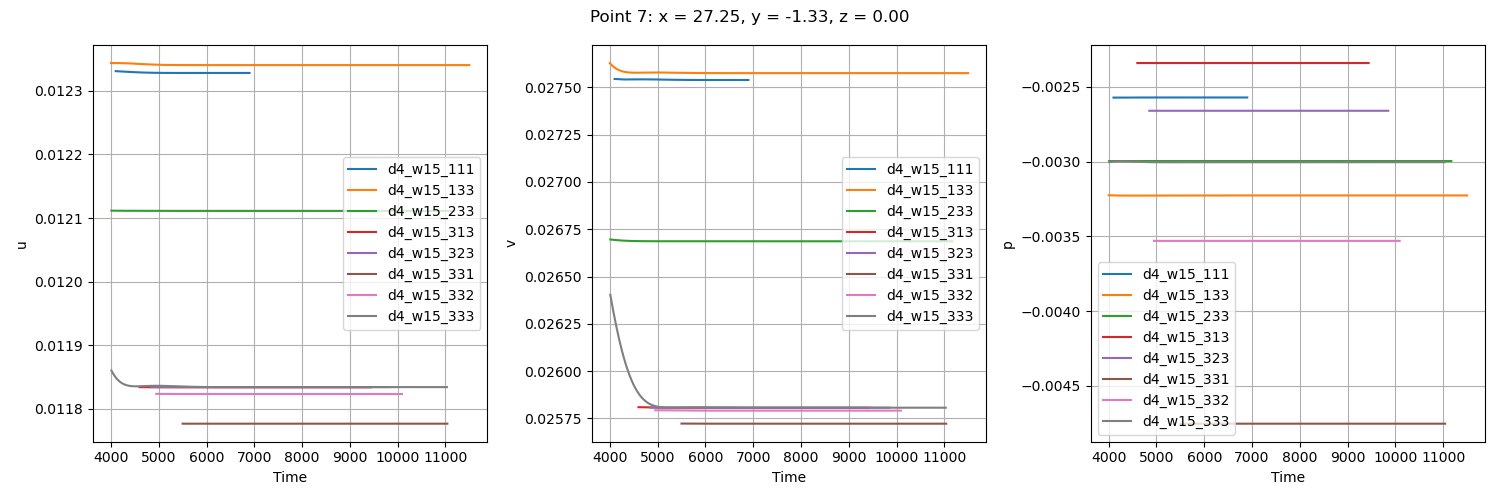
\includegraphics[width=\linewidth]{Images/point8.png}
\end{frame}
\begin{frame}
	\frametitle{Results}
	Point 9:

	\centering
	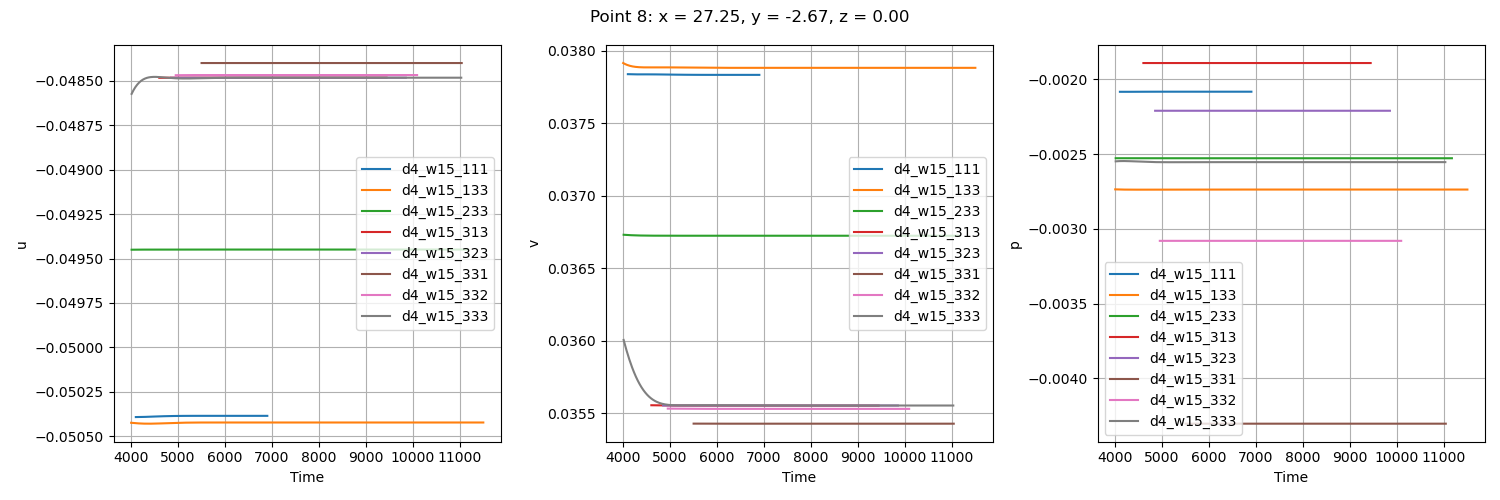
\includegraphics[width=\linewidth]{Images/point9.png}
\end{frame}
\begin{frame}
	\frametitle{Results}
	Point 10:

	\centering
	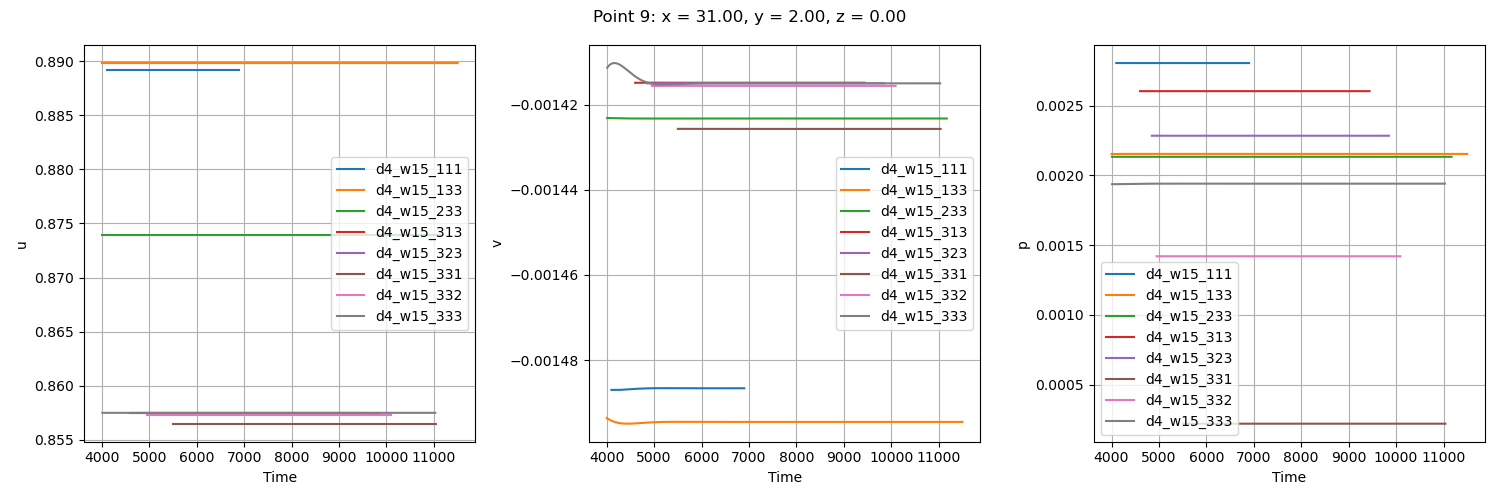
\includegraphics[width=\linewidth]{Images/point10.png}
\end{frame}
\begin{frame}
	\frametitle{Results}
	Point 11:

	\centering
	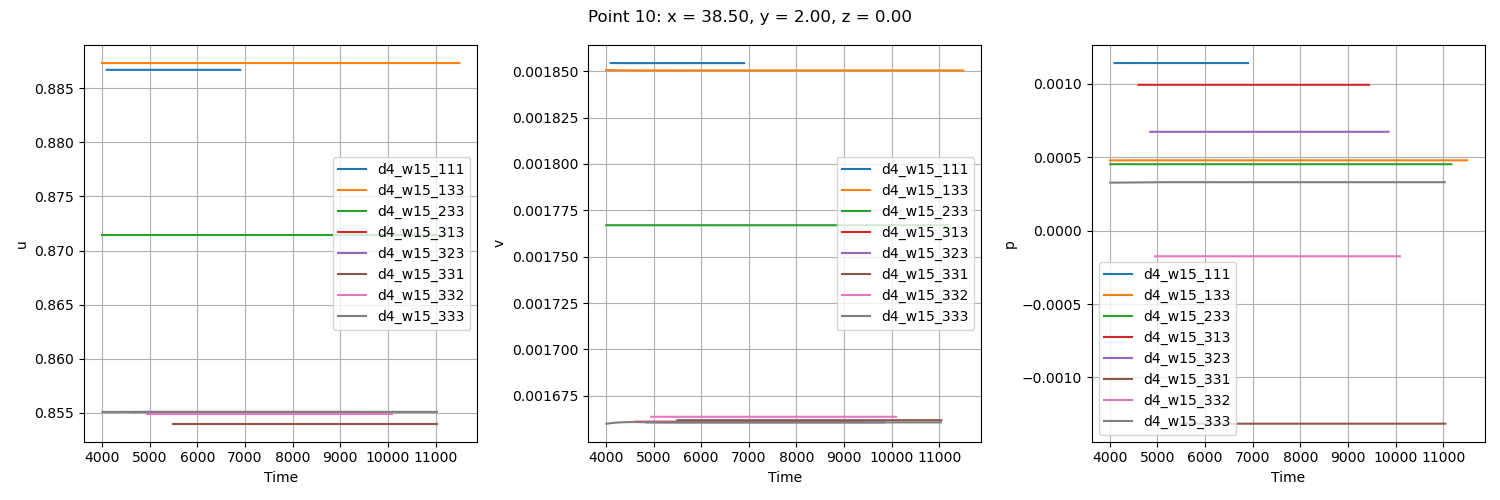
\includegraphics[width=\linewidth]{Images/point11.png}
\end{frame}
\begin{frame}
	\frametitle{Results}
	Point 12:

	\centering
	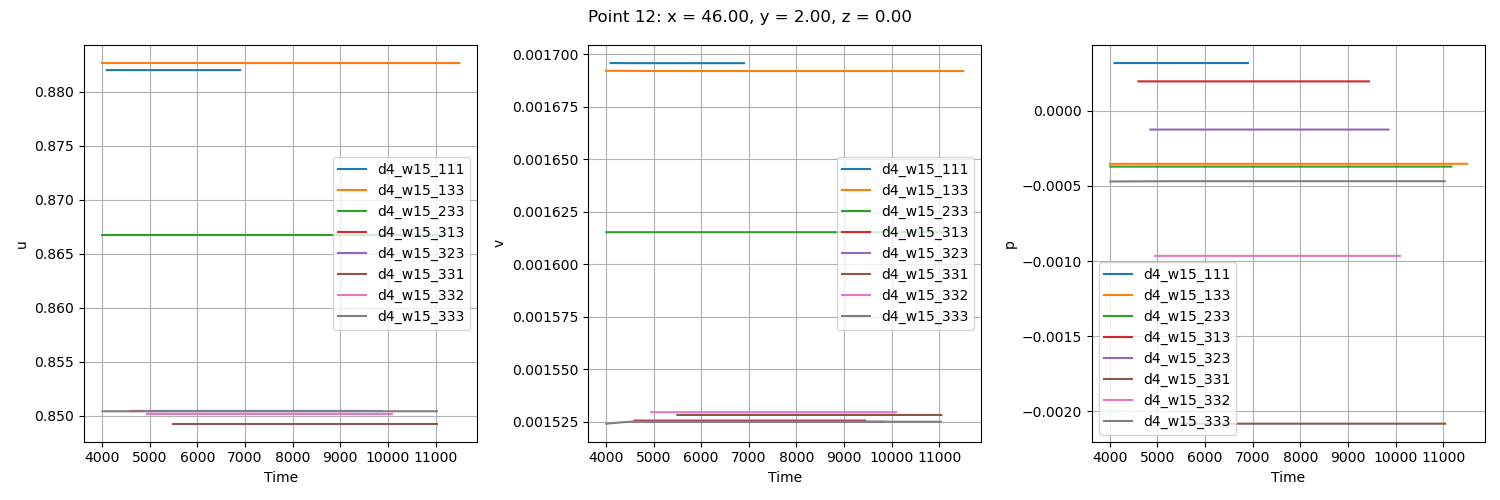
\includegraphics[width=\linewidth]{Images/point12.png}
\end{frame}
\begin{frame}
	\frametitle{Conclusions}

	\begin{itemize}
		\item The distance after the gap is not that important for $u$ and $v$.
		\item The pressure is the most sensitive to the domain size.
	\end{itemize}

	\centering
	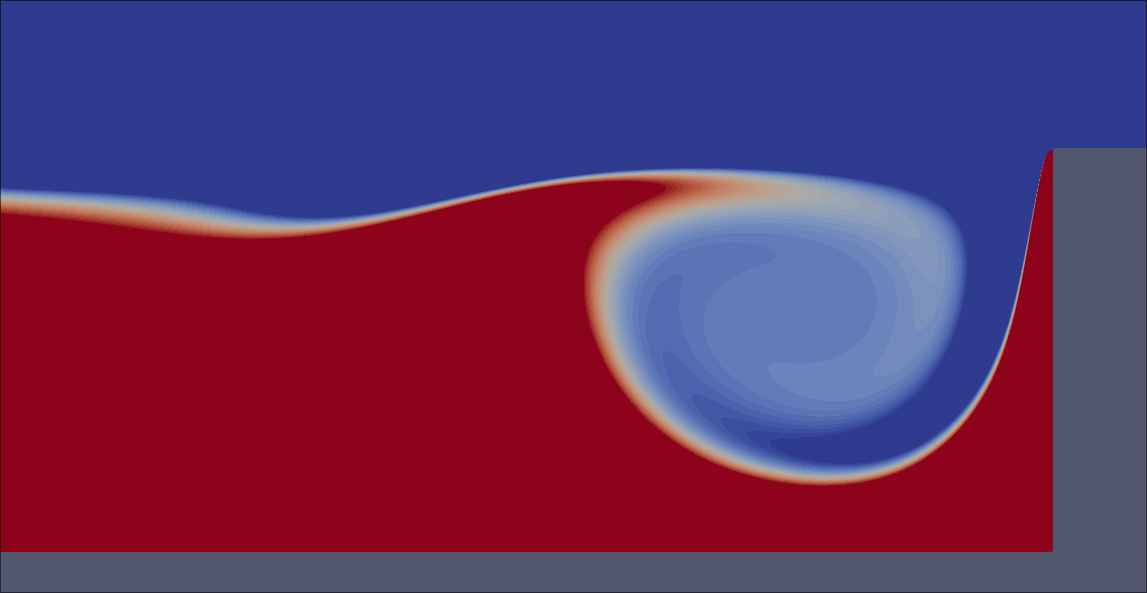
\includegraphics[width=0.5\linewidth]{Images/vortex.png}

	{\small The resolution of the vortex was decent }

\end{frame}

\end{document}
